\documentclass[a4paper,10pt]{article}

\usepackage[utf8]{inputenc} %
\usepackage[english]{babel}
\usepackage{fontenc}
\usepackage{graphicx}
\usepackage{amsfonts}
\usepackage{hyperref}
\usepackage{amssymb}
\usepackage{fullpage}
\usepackage[ruled,vlined,linesnumbered]{algorithm2e}
\usepackage{float}
\usepackage{amsthm}
\usepackage{amsmath}
\usepackage{amssymb}
\usepackage{mathrsfs}
\usepackage{enumerate}
\providecommand{\SetAlgoLined}{\SetLine}
\providecommand{\DontPrintSemicolon}{\dontprintsemicolon}
\author{Projet GL}
\date{Octobre 2013}
\title{Répartion Groupe
}
\theoremstyle{definition}
\newtheorem{lemma}{Lemme}
% \newtheorem{proposition}{Propriété}[chapter]
% \newtheorem{definition}{Définition}[chapter]
% \newtheorem{example}{Exemple}[chapter]
% \newtheorem{cor}{Corollaire}[chapter]
% \newtheorem{theorem}{Théorème}[chapter]
\theoremstyle{definition}
\usepackage{tikz}
\usetikzlibrary{arrows}
\usepackage{fullpage}
\usepackage{empheq}
 
% Command "alignedbox{}{}" for a box within an align environment
% Source: http://www.latex-community.org/forum/viewtopic.php?f=46&t=8144
\newlength\dlf  % Define a new measure, dlf
\newcommand\alignedbox[2]{
% Argument #1 = before & if there were no box (lhs)
% Argument #2 = after & if there were no box (rhs)
&  % Alignment sign of the line
{
\settowidth\dlf{$\displaystyle #1$} 
    % The width of \dlf is the width of the lhs, with a displaystyle font
\addtolength\dlf{\fboxsep+\fboxrule} 
    % Add to it the distance to the box, and the width of the line of the box
\hspace{-\dlf} 
    % Move everything dlf units to the left, so that & #1 #2 is aligned under #1 & #2
\boxed{#1 #2}
    % Put a box around lhs and rhs
}
}
\theoremstyle{remark}
% \newtheorem{req}{Remarque}[chapter]
% \newtheorem{nota}{Notation}[chapter]

\tikzset{
    punkt/.style={
           rectangle,
           rounded corners,
           draw=black, very thick,
           text width=5em,
           minimum height=2em,
           text centered},
    punkt2/.style={
           rectangle,
           draw=pink, very thick,
           text width=5em,
           minimum height=2em,
           text centered},
  treenode/.style = {align=center, inner sep=0pt, text centered,
    font=\sffamily},
  arn_n/.style = {treenode, circle , white, font=\sffamily\bfseries, draw=black,
    fill=black, text width=1.5em},% arbre rouge noir, noeud noir
  arn_r/.style = {treenode, circle , red, draw=red, 
    text width=1.5em, very thick},% arbre rouge noir, noeud rouge
  arn_x/.style = {treenode, rectangle, draw=black,
    minimum width=1em, minimum height=1em},% arbre rouge noir, nil
  arn_b/.style = {treenode, circle , blue, draw=blue, 
    text width=1.5em, very thick},
  arn_g/.style = {treenode, circle , green, draw=green, 
    text width=1.5em, very thick},
  arn_y/.style = {treenode, circle , yellow, draw=yellow, 
    text width=1.5em, very thick},
    arn_pu/.style = {treenode, circle , purple, draw=purple, 
    text width=1.5em, very thick},
    arn_pi/.style = {treenode, circle , pink, draw=pink, 
    text width=1.5em, very thick},
    arn_rb/.style = {treenode, circle , red, draw=red, 
    text width=2.5em, very thick}
    }% arbre rouge noir, noeud rouge}
    \begin{document}
    \maketitle
     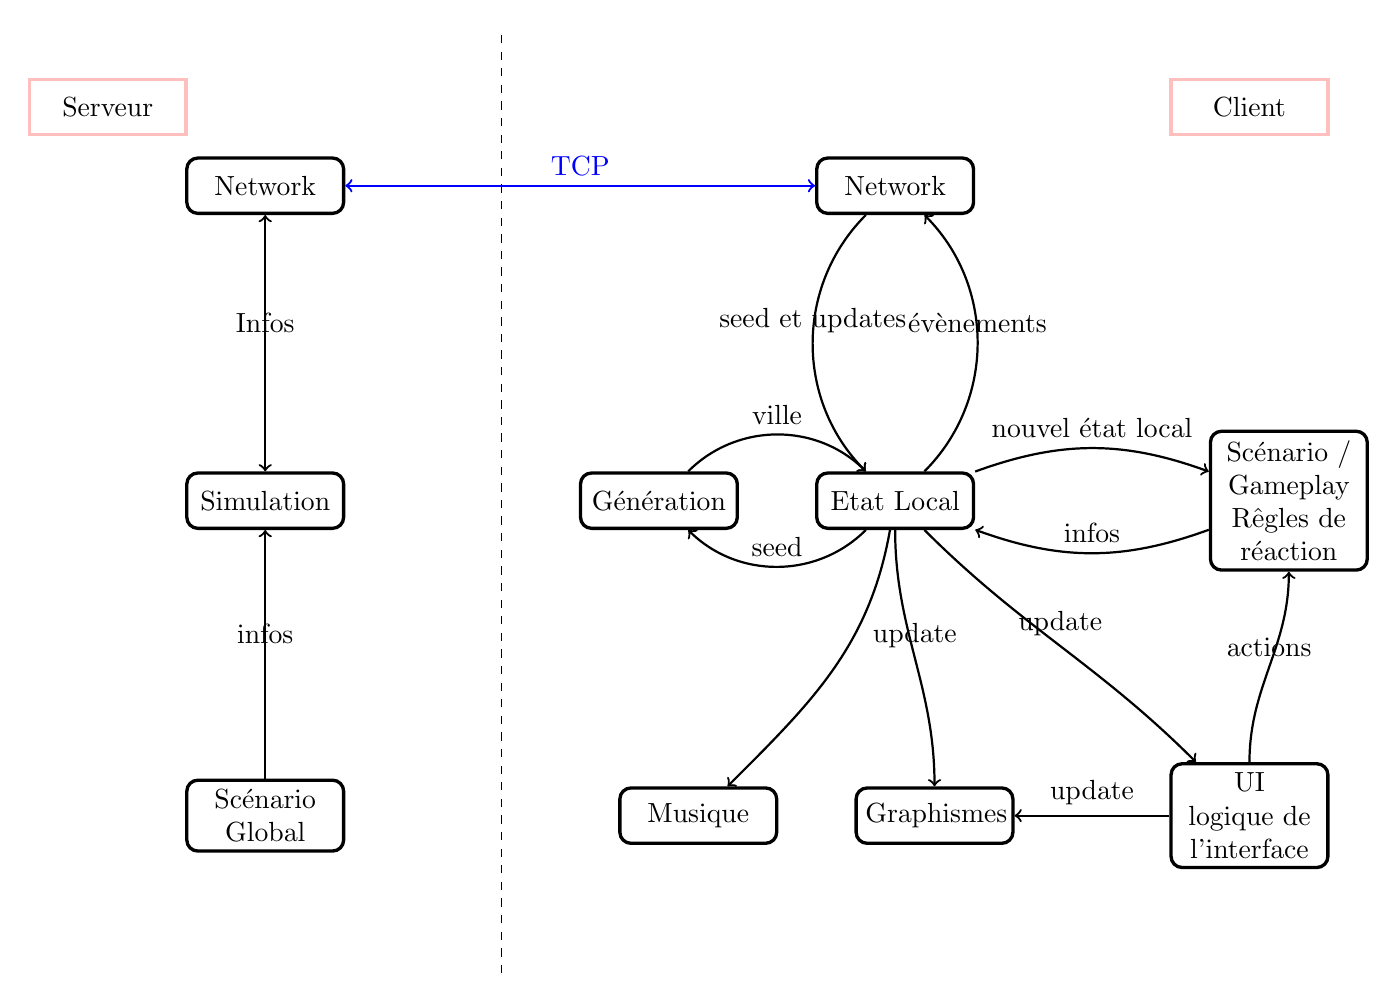
\begin{tikzpicture}
      \node[punkt] (0) at (3,0) {Etat Local};
      \node[punkt] (1) at (0,0) {Génération};
      \node[punkt] at (0.5,-4) (2) {Musique};
      \node[punkt] at (3.5,-4) (3) {Graphismes};
      \node[punkt] at (7.5,-4) (4) {UI \\ logique de l'interface};
      \node[punkt] at (8,0) (5) {Scénario / Gameplay \\ Rêgles de réaction};
      \node[punkt] at (3,4) (6) {Network};
      \node[punkt] at (-5,0) (7) {Simulation};
      \node[punkt] at (-5,-4) (8) {Scénario Global};
      \node[punkt] at (-5,4) (10) {Network};
      \node[punkt2] at (7.5,5) {Client};
      \node[punkt2] at (-7,5) {Serveur};
      \draw[-,black,dashed] (-2,-6) -- (-2,6);
      \draw[->,black,thick] (1) to[out=45,in=135] node [midway,above] {ville} (0);
      \draw[->,black,thick] (0) to[out=225,in=-45] node [midway,above] {seed} (1);
      \draw[->,black,thick] (0) to[out=260,in=45] (2);
      \draw[->,black,thick] (0) to[out=270,in=90] node [midway,above] {update} (3);
      \draw[->,black,thick] (0) to[out=-45,in=135] node [midway,above] {update} (4);
      \draw[->,black,thick] (0) to[out=20,in=160] node [midway,above] {nouvel état local} (5);
      \draw[->,black,thick] (5) to[out=200,in=-20] node [midway,above] {infos} (0);
      \draw[->,black,thick] (4) to[out=90,in=-90] node [midway,above] {actions} (5);
      \draw[->,black,thick] (4) to[out=180,in=0] node [midway,above] {update} (3);
      \draw[->,black,thick] (0) to[out=45,in=-45] node [midway,above] {évènements} (6);
      \draw[->,black,thick] (6) to[out=-135,in=135] node [midway,above] {seed et updates} (0);
      \draw[<->,blue,thick] (6) to[out=180,in=0] node [midway,above] {TCP} (10);
      \draw[<->,black,thick] (10) to[out=-90,in=90] node [midway,above] {Infos} (7);
      \draw[->,black,thick] (8) to[out=90,in=-90] node [midway,above] {infos} (7);

      
      
     \end{tikzpicture}

    \end{document}
